\chapter{Time Is Valuable}

These notes follow Jim Rohn's lecture as preserved in a curated LazyingArt LLC playlist rather than a clean institutional course. Although the video title emphasizes time, the lecture first builds a law of deserving, then widens into service, leadership, personal development, patience, and finally a concrete algorithm for solving problems on paper. The mathematics here is therefore structural rather than quantitative: the displayed formulas compress a sequence of practical rules, repeated examples, and disciplined transitions in the order in which the lecture develops them.

\paragraph{Heuristic status.}
No validated blackboard frames survive for this lecture, so every displayed formula and diagram below is transcript-backed or a cautious reconstruction of the lecture's process logic. They should be read as companion notes to the spoken argument, not as formal economics or psychology.

\section{Enlightened Self-Interest and the Law of Deserving}

The lecture opens by naming its first subject: enlightened self-interest. Rohn begins not with altruism in the abstract, but with the plain fact that we are interested in our own survival and success. The first operation is therefore definitional. Self-interest is not denied. It is constrained, educated, and redirected.

\begin{equation}
\text{self-interest} \rightarrow \{\text{survival},\text{success}\}.
\end{equation}

The qualifying word is the essential one:
\begin{equation}
S_{\mathrm{enl}}=\text{self-interest constrained so that everybody wins and no one loses}.
\end{equation}

A short stretch of transcript is noisy at the exact point where Rohn moves from this opening idea to the deeper law, but the secure content is clear enough. The structure of things, or in his language the design of life and God, does not grant outcomes merely because we need them. It grants outcomes when we have qualified for them.

\begin{definition}
In the lecture's operational sense, deserving does not mean moral superiority. It means that some qualifying action has begun and has been sustained far enough that a result is now due.
\end{definition}

This gives the chapter its governing maxim:
\begin{equation}
\text{we get not what we need, but what we deserve}.
\end{equation}

Rohn immediately strips the claim of sentimental vagueness. He does not say first that deserving is a matter of inward feeling. He says that it is attached to action, sequence, and law. That is why the lecture can become mathematical at all. It is not merely saying that better people get better things. It is saying that certain processes lead to certain results.

\section{Plant, Knock, Search, Ask}

The lecture now tightens the governing maxim by repeating it four times. These are not four unrelated sayings. They are four versions of the same rule.

\begin{align}
\text{need} &\not\Rightarrow \text{harvest}, &
\text{planting} &\Rightarrow \text{deserved reaping}, \\
\text{continual knocking} &\rightarrow \text{open doors}, &
\text{searching} &\rightarrow \text{finding}, \\
\text{asking} &\rightarrow \text{qualification for answers}. &&
\end{align}

The agricultural example is the first and clearest. We do not reap in the fall because we need the harvest. We reap because the planting has been done. Rohn insists that reaping is reserved for the planters. The form of the statement matters. Reaping is not treated as random reward. It is treated as the lawful consequence of an earlier step.

The same structure is then carried into opportunity. Open doors are not granted to mere need. They are found by those who continually knock. And once that transition has been made, the lecture can move again: finding is reserved for the searchers, and answers belong to those who keep asking. The lecture wants us to feel a pattern rather than memorize four proverbs.

\begin{figure}[t]
\centering
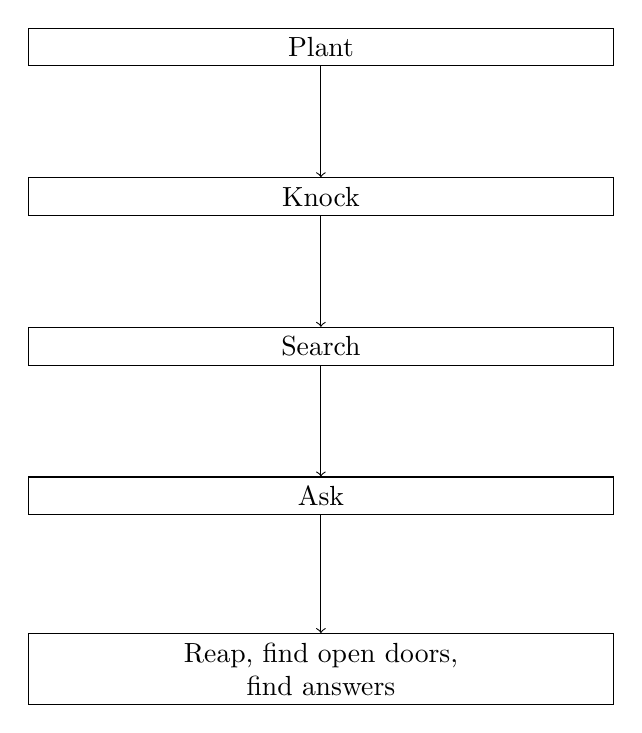
\begin{tikzpicture}[x=1cm,y=1cm]
\node[draw,align=center,text width=7.2cm] (a) at (0,0) {Plant};
\node[draw,align=center,text width=7.2cm] (b) at (0,-1.9) {Knock};
\node[draw,align=center,text width=7.2cm] (c) at (0,-3.8) {Search};
\node[draw,align=center,text width=7.2cm] (d) at (0,-5.7) {Ask};
\node[draw,align=center,text width=7.2cm] (e) at (0,-7.9) {Reap, find open doors,\\find answers};
\draw[->] (a) -- (b);
\draw[->] (b) -- (c);
\draw[->] (c) -- (d);
\draw[->] (d) -- (e);
\end{tikzpicture}
\caption{A transcript-backed deserve-logic ladder. The lecture's repeated examples are parallel instances of one rule: action qualifies outcome.}
\end{figure}

The lecture then adds a local seminar application. Those who have come to the event have already entered the search process. They got on airplanes, got in cars, and arrived looking. Therefore they are now in position to receive plans, answers, and imagination for future action. The result is not accidental inspiration. It is the continuation of the same logic.

\subsection{Question \& Answer}

The natural question is immediate: if harvest, opportunity, and answers are all deeply needed, why are they not given merely because they are needed?

The lecture's answer is that need indicates lack, but not yet qualification. The structure may be summarized as
\begin{equation}
N \not\Rightarrow R, \qquad N + Q \Rightarrow D \Rightarrow R,
\end{equation}
where \(N\) denotes need, \(Q\) the qualifying process, \(D\) deserving, and \(R\) the result. In the lecture's own examples, planting, knocking, searching, and asking are the forms that \(Q\) takes. Need may motivate the process, but it is not the process.

\section{Need, Seed, and the Process of Deserving}

Having established the law abstractly, the lecture turns to social mechanism. This is an important change in level. We are no longer in the region of maxims alone. We are now being shown how a person begins to move from bare need into qualification.

A useful compression of the lecture's central reconstruction is
\begin{equation}
\text{deserving}=\text{qualifying action sustained over time}.
\end{equation}

Rohn's welfare example should be read in that narrow sense. He does not claim that painting a fence is equivalent in market value to a welfare check. He says instead that a small act can begin a process. That distinction matters.

\paragraph{Worked example: the beginning of deserving.}
Let \(N_0\) be a state of need and let \(A_n\) denote the \(n\)-th qualifying act. Then the lecture's example may be written as
\begin{align}
N_0 &\not\Rightarrow \$450, \\
A_1 &= \text{paint the door and the fence}, \\
D_1 &= D_0 + A_1, \\
A_2 &= \text{clear the weeds and cultivate the garden}, \\
D_2 &= D_1 + A_2.
\end{align}
The point is not that \(A_1\) or \(A_2\) is worth a fixed sum. The point is that
\begin{equation}
D_{n+1}=D_n + A_{n+1}
\end{equation}
is the lecture's stepwise picture of renewal. A new life emerges by stages, not by mere complaint.

The same rule appears again at home. A child says, ``I need ten dollars.'' Rohn's answer is that this is not how the vault opens. The better question is: how could I earn ten dollars? In the lecture's symbolic language,
\begin{equation}
\text{need} \not\Rightarrow \$10, \qquad \text{earn}(\$10) \Rightarrow \text{vault opens}.
\end{equation}

The field and the marketplace then become two versions of the same rebuttal. One cannot walk out to the field and announce a need for crops while bringing no seed. And one cannot disclose bare need to the marketplace and expect resources to flow. The lecture's blunt formula is one of its sharpest:
\begin{equation}
\text{take your seed to the marketplace, not your need}.
\end{equation}

This is then unpacked more carefully:
\begin{equation}
\text{marketplace interest}
=
\{\text{seed},\text{willingness},\text{discipline},\text{eagerness},\text{vitality},\text{work ethic}\}.
\end{equation}

The meaning is straightforward. Need may be psychologically real, but it is not the object the marketplace responds to. The marketplace responds to the signs that value can be created.

\subsection{Question \& Answer}

The lecture now raises a better question than ``How do I get what I need?'' It asks: what process should I begin engaging in to deserve good health, good relationships, prosperity, and enterprise?

The answer is deliberately modest. One does not begin with the full finished result. One begins with the first qualifying act. The transition is
\begin{equation}
\text{state of need} \rightarrow \text{first disciplined act} \rightarrow \text{process of deserving}.
\end{equation}

That is why the lecture prefers seed to need, earning to requesting, and cultivation to complaint. The key word is \emph{begin}. Deserving is not first a trophy. It is a process we enter.

\section{Giving, Service, Greatness, and Small Beginnings}

The lecture then returns explicitly to enlightened self-interest. The wish to receive is self-interest; Rohn does not deny it. But enlightened self-interest understands sequence.

\begin{align}
\text{if you wish to receive, you must give}, \\
\text{receiving is reserved for those who give}, \\
\text{giving} \rightarrow \text{receiving process begins}.
\end{align}

This is Rohn's explanation of the maxim that it is better to give than to receive. He is not merely making a moral compliment to generosity. He is stating a process order. Giving is better in the same sense that planting is better than reaping at the beginning of the cycle: it initiates what later returns.

The lecture then asks the larger question: how do we become great? The answer is not self-enclosure, even though self-preservation has its place. Greatness comes by extending service outward.
\begin{equation}
\text{service to many} \rightarrow \text{greatness}.
\end{equation}

This section of the transcript contains some duplication, but the doctrinal line is steady. We do not reach abundance by solving only our own problems. We begin the process of greatness when we help solve other people's problems and help find answers for them.

The next escalation is from greatness in general to leadership and stewardship in particular. How does one become ruler over many? How does one manage large resources or lead a vast movement? The answer is not dramatic. It is miniature.
\begin{align}
\text{faithful with little} &\rightarrow \text{qualified for much}, \\
\text{discipline with small amounts} &\rightarrow \text{qualification for riches}, \\
\text{few listeners treated faithfully} &\rightarrow \text{qualification to speak to many}.
\end{align}

This is one of the lecture's strongest structural claims. The small paycheck, the small team, and the small audience are not embarrassments. They are tests. If a person does not know where the few dollars go, the lecture says, that very disorder disqualifies him from stewardship over the larger amount. Likewise, if a speaker is indifferent when there are only a few listeners, he is not yet being shaped for the larger crowd.

Rohn then supplies his own case. He did not begin by speaking to thousands. He began by trying, awkwardly, to translate life-changing ideas for a few. This matters for the logic of the chapter. Qualification does not descend fully formed; it begins in fidelity to the small scene now in front of us.

\section{Personal Development as Refinement}

Only after the law of deserving has been driven through work, service, and leadership does the lecture widen into a broader account of personal development. The emphasis here is refinement: we are to give ourselves a chance to change, revise our philosophy, and reconsider what we once thought final.

The lecture states this almost as an opening condition for later opportunity:
\[
\text{re-evaluation} \rightarrow \text{new door}.
\]

The point is not indecision for its own sake. It is that rigid attachment to an earlier self can prevent discovery. Change of philosophy and change of direction are not betrayals of seriousness; they are often its proof.

The library then enters as a physical sign of this seriousness. We are urged to let the library testify to our dedicated interest in accelerated personal development. Read what must be read, hear what must be heard, see what must be seen. The seminar itself is then described as a stopping station and a catalyst. We are asked to sit, listen, take notes, ponder, and work, so that the refinement has already begun before we return home.

The formal summary of this block is compact:
\begin{equation}
\text{good ideas} + \text{good plans} + \text{time-handling} \rightarrow \text{steps to success}.
\end{equation}

Rohn makes the sequence dynamic rather than static:
\begin{equation}
\text{one good idea} \rightarrow \text{next idea} \rightarrow \text{further acceleration}.
\end{equation}

This is an important piece of the lecture's pacing. The seminar is not presented as a container of isolated insights. It is presented as a device for starting a chain. One good idea does not merely solve one problem. It makes later ideas more accessible. That is why the lecture expects multiplication: two times, three times, five times more than we had thought possible.

The plans named here are concrete and various: a health plan, a family plan, a marriage plan, a plan for using the day, a plan for meeting the right people over the right amount of time, and a plan for lifestyle. Rohn's point is that a life left undesigned tends to drift. The plan is not a decorative spreadsheet laid over life after the fact. It is a means of giving life shape before circumstances give it one for us.

\section{Time, Patience, and the Rule That Most Will}

Now the lecture reaches the title theme directly. All the preceding processes require time. One cannot have a law of sowing and reaping without seasons, and one cannot have growth in people without patience.

\begin{equation}
\text{time} + \text{patience} \rightarrow \text{growth, learning, and change}.
\end{equation}

Rohn's examples proceed from the crop to the business, from the business to the family, and from the family to the self. Projects need time. People need time. Children, spouses, co-workers, and independent personalities require patience. The metaphor of herding cats is comic, but its structural use is serious: coordination among free persons is slow and difficult.

The lecture then makes the crucial inward turn. We must have patience with ourselves. Learning, change, and refinement do not happen at identical speeds for all people. The image of learning to tie one's shoes is deliberately elementary. The point is not that later growth is childish. The point is that all growth has this form: repetition, frustration, and gradual mastery.

The social extension of patience is then given in a memorable rule:
\begin{equation}
\text{usually enough good people} \rightarrow \text{social stability}.
\end{equation}

Rohn phrases this as ``most will'' or ``enough will.'' He does not claim that every person in a community, government, school, or institution will do the right thing. He claims instead that in a civilized society enough people usually will. That is the working condition for order.

The Sodom-and-Gomorrah story functions here as an exception, not as a detour. Abraham keeps lowering the threshold---fifty, forty, thirty, ten---and the city still fails the test. Rohn's point is not to linger over destruction. It is to show that complete breakdown is the exception to the more usual rule. Most of the time enough people keep the structure standing.

We should be careful not to formalize this beyond the lecture. ``Most will'' is not a probability theorem. It is a practical confidence condition. It tells us why patience is rational in ordinary life.

\section{Thinking on Paper: Solving Problems}

The lecture closes by becoming methodical. After broad claims about deserving, service, and patience, we arrive at an actual procedure. This final section is the clearest algorithm in the talk.

The first move is to relocate the problem:
\begin{equation}
\text{problem in head} \rightarrow \text{problem on paper} \rightarrow \text{sortable object of thought}.
\end{equation}

The justification is immediately psychological. The mind is busy. It mixes together fear, haste, memory, and fragments. Once the problem is on paper, we can inspect it. We can ask whether we have described all of it. And only then can we begin prescribing something for it.

\subsection{Question \& Answer}

The natural question is this: how do we solve a problem when the mind is too busy to sort it out?

The lecture's answer is to think on paper. A page is divided in two. On the left we describe the problem; on the right we write answers and solutions. This is not a literary recommendation. It is an analytic one.

\begin{figure}[t]
\centering
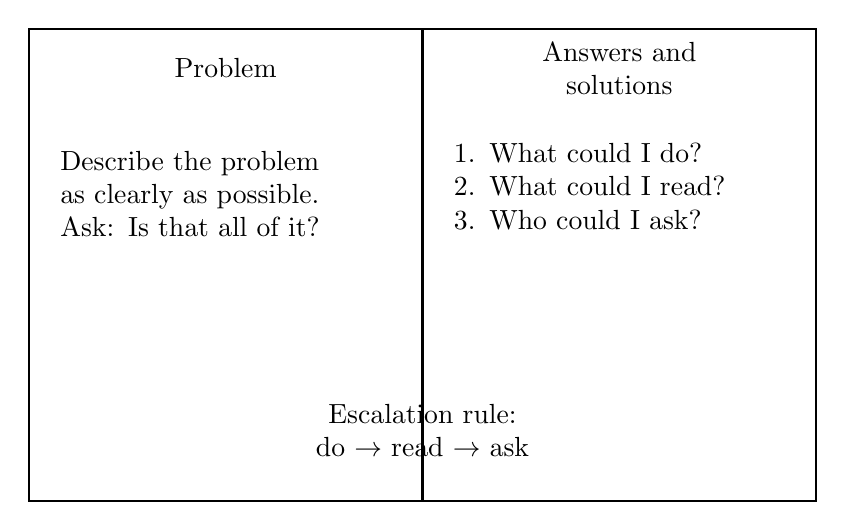
\begin{tikzpicture}[x=1cm,y=1cm]
\draw[thick] (0,0) rectangle (10,-6);
\draw[thick] (5,0) -- (5,-6);
\node[align=center] at (2.5,-0.5) {Problem};
\node[align=center] at (7.5,-0.5) {Answers and\\solutions};

\node[align=left,text width=4.2cm] at (2.5,-2.1) {Describe the problem\\as clearly as possible.\\Ask: Is that all of it?};

\node[align=left,text width=4.2cm] at (7.5,-2.0) {1. What could I do?\\2. What could I read?\\3. Who could I ask?};

\node[align=center,text width=8.5cm] at (5,-5.1) {Escalation rule:\\do $\rightarrow$ read $\rightarrow$ ask};
\end{tikzpicture}
\caption{A transcript-backed page layout for the lecture's problem-solving method. The figure is an editorial reconstruction from spoken instructions rather than from board evidence.}
\end{figure}

A compact reconstruction of the working papers is
\begin{align}
W_0(X) &= \text{state the problem } X \text{ as clearly as possible}, \\
W_1(X) &= \text{ask: Is that all of it?}, \\
U(X) &= \text{list what I could do}, \\
R_b(X) &= \text{list what I could read or research}, \\
A_s(X) &= \text{list who I could ask}.
\end{align}

The lecture then imposes an order:
\begin{equation}
\text{do} \rightarrow \text{read} \rightarrow \text{ask}.
\end{equation}

This order matters. We do not ask first. We try first. If the first list fails, we search and research. If research still does not answer the question, then we ask someone else. The lecture reinforces the second stage with the same old law:
\begin{equation}
\text{search/research} \rightarrow \text{find}.
\end{equation}

The deeper reason for postponing the third step is not pride. It is development. If we immediately borrow every answer, we fail to build internal capacity.
\begin{align}
\text{trying first yourself} &\rightarrow \text{mental and emotional muscle}, \\
\text{helping yourself first} &\rightarrow \text{others respond more quickly with help}.
\end{align}

This is why Rohn asks us to bring working papers when we finally ask. A person who says, ``I have tried this, I have read this, and I still do not see the answer,'' is easier to help than a person who has done nothing. More than that, the first person is already stronger, because the attempt itself has built discipline. The lecture's final warning is implicit: there may come a day when there is no one else to ask.

\section{Summary}

The lecture begins with enlightened self-interest and ends with a sheet of working paper. Between those two points it builds one coherent law. Need alone does not entitle us to a result. Qualification, action, and sustained process do. Planting precedes reaping. Knocking precedes open doors. Searching precedes finding. Asking precedes answers.

From there the law broadens. Seed matters more than disclosed need in the marketplace. Giving begins receiving. Service to many leads to greatness. Faithfulness with little prepares stewardship over much. Good ideas require good plans, and both require time. Patience makes growth possible because most of the time enough good people make life workable. Finally, when life becomes knotted, we take the knot out of the head and put it on paper.

The chapter's mathematics is modest, but its structure is rigorous. It is a lecture about sequence: what must come first, what may follow, and why no durable result can be had by trying to skip the qualifying step.